\documentclass[12pt]{beamer}

\mode<presentation> {
	
	
	%\usetheme{Madrid}
	%\usepackage{times}
	\renewcommand{\familydefault}{\rmdefault}
	\usetheme{CambridgeUS}
	\usepackage[latin1]{inputenc}
	\usefonttheme{professionalfonts}
	\usepackage{times}
	\usepackage{tikz}
	\usepackage{amsmath}
	\usepackage{verbatim}
	\usepackage{enumerate}
	\usepackage{setspace}
	\usetikzlibrary{arrows,shapes}
	\usepackage{amsmath}
	\usepackage{eurosym}
	\usepackage{framed}
	\usepackage{extarrows}

}

\usepackage{graphicx}
\usepackage{booktabs}
\usepackage{url}

%----------------------------------------------------------------------------------------
%	TITLE PAGE
%----------------------------------------------------------------------------------------


\title{Approximation of JPY/USD exchange rate by RBF neural networks}

\author[Group ID: No.11]{Instructor: Group ID: No.11} % Your name
\institute[]{
	\textsl{Project ID: No.9}
}
\date[July 20$^{th}, 2016$]{} % Date, can be changed to a custom date







\begin{document}
	
\begin{frame}
	\titlepage
\end{frame}


\begin{frame}
	\frametitle{Outline}
	\tableofcontents
\end{frame}

\section{Introduction}

\begin{frame}
	\frametitle{Introduction}
	\quad   Neural network is able to approach any functions infinitely in theory .And
there is a good effect in forecasting field with neural network .With the ability
of numeric approaching and memory , it can identify the inherence pattern of
exchange rate sequence according to the historic data.At the beginning.
\end{frame}






\section{Data source}
\begin{frame}
	\frametitle{Data source}
	 \quad Data selection, first of all, to determine the data sampling rules based on time series, extract the relevant data from the original data of the database as a
sample or forecast data. Data selection includes training sample selection and
prediction data selection, the two are different from the prediction data
selection process only select the network input data and the sample selection
and output data.We get the forward exchange data,spot exchange rate from
wind.
\end{frame}


\section{Procedure}

\begin{frame}
	\frametitle{Procedure}
	The choice of the original data need to be processed into a neural network processing in the form of data preprocessing will be reduced to a specific range of data $\left[ -1,1\left] $  and $\left[ 0,1\left] $ is commonly used in the specification range. The predictor allows users to choose through the visual interface. According to the expert guidance and in the actual test and comparison, we in the experiment of the original data are mapped to the $\left[ 0,1\left] $ range\\

\end{frame}



\section{Plots}
\begin{frame}
\frametitle{Plots}

\begin{figure}
  \centering
  % Requires \usepackage{graphicx}
  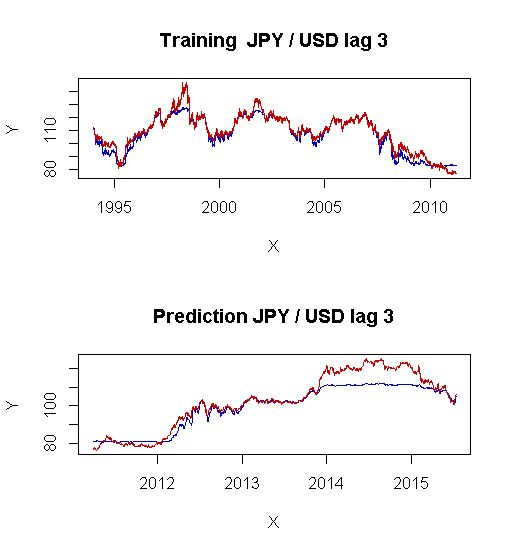
\includegraphics[width=200pt]{picture.png}\\
\end{figure}
\


\end{frame}


	
	
\end{document}
